\documentclass[UTF8]{ctexart}

\usepackage{subfiles}  

%下面的语句, 引入你的头部设置文件
\usepackage{C:/phpStorm_proj/02_myself_ID_EGO/+100_latex_all_math_sel/myPreamble} 
%必须是绝对路径,才能让各个tex在单独编译时使用到

\title{文件名}


%---------------------------------


\begin{document}
	\tableofcontents % 生成目录
	\date{} % 若不写这句, 则默认也会渲染出日期, 所以我们要手动赋空值
	\maketitle  %这行代码, 让你前面的 title, author, date生效
	
	\section{连续型 : 均匀分布 $f(x)=\frac{1}{b-a}\ (a\leq x\leq b)	$ }
	
	``均匀分布 Uniform Distribution"也叫``矩形分布", 它是对称概率分布, 即\textbf{在相同长度间隔的分布概率, 是等可能的.} \\
	
	``均匀分布"由两个参数a和b定义, 它们是数轴上的最小值和最大值. 通常缩写为 U(a,b). \\
	
	其``概率函数"是: 
		$	f\left( x \right) =\left\{ \begin{array}{l}
		\dfrac{1}{b-a}\ \ \ \ a\leq x\leq b\\
		0\ \ \ \ \ \  \ \ else\\
	\end{array} \right. 	$ 
	记作: $X \sim U(a,b]$ \\
	
	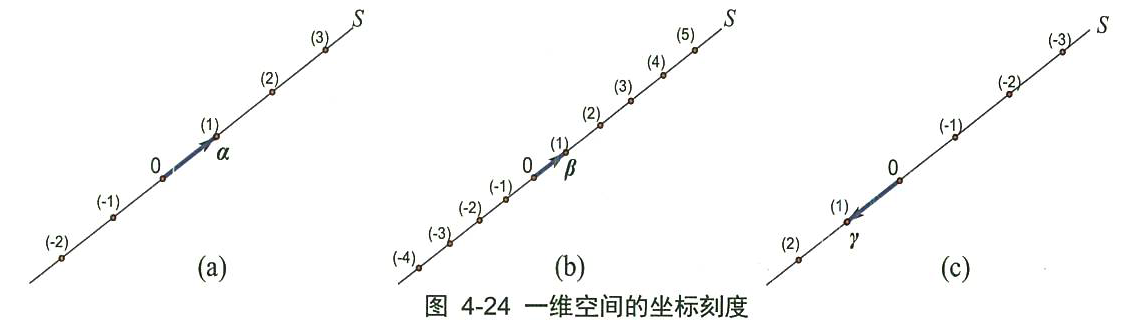
\includegraphics[width=0.4\textwidth]{/0172.png} \\
	
	其``累加函数 F(x)"是 : \\
	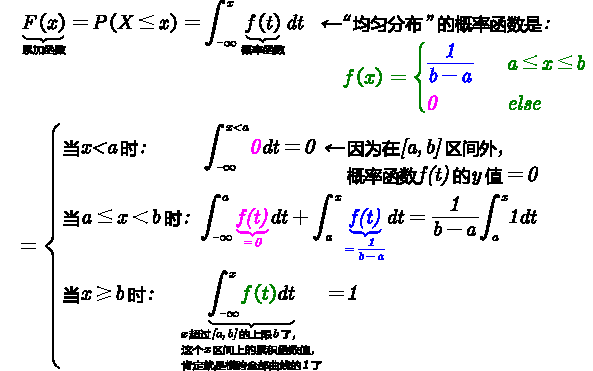
\includegraphics[width=0.75\textwidth]{/0171.pdf} \\

	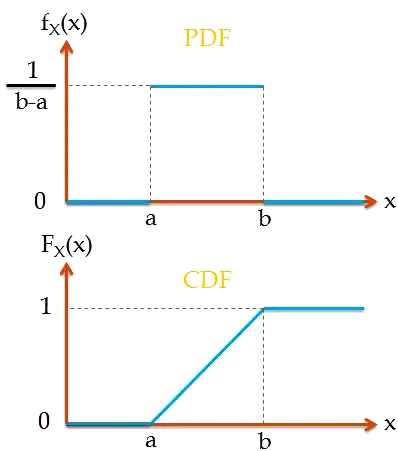
\includegraphics[width=0.4\textwidth]{/0173.png} \\
	
	
	
	
	
	
	\subsection{若 [c,d]区间 $\in$ [a,b]区间中, 则有: $ 
		 P\{c \leq x \leq d\} = \int_c^d \dfrac{1} {b-a} dt = \dfrac{d-c} {b-a}$}
	
	对 $X \sim U[a,b]$, 若有[c,d]区间, 是包含在 [a,b]区间里面的, 即 $ [c,d] \in [a,b]$, 则 x落在c和d 之间的概率, 就是 $= P\{c \leq x \leq d\} = \int_c^d \dfrac{1} {b-a} dt = \dfrac{d-c} {b-a}$ \\
	
	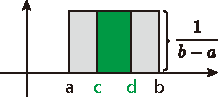
\includegraphics[width=0.35\textwidth]{/0174.pdf} \\
	
	也就是说, ``均匀分布" 在[a,b]区间的概率值, 是一个矩形. 所以其里面的 [c,d]区间的概率, 也是一个小矩形. 这两个矩形的面积之比, 就是它们相应的``长或宽的长度"对比. \\
	
	
	\begin{myEnvSample}
	某公交车站, 从7点开始(其实这个时间点是个障眼法, 跟我们解题毫无关系), 每15分钟开一班车. \\
	乘客会在 7:00-7:30之间到达车站, 符合``均匀分布". \\
	那么这半个小时区间的首尾值, 就是区间a和b的值了. 	即: [a=0, b=30] \\
	根据``均匀分布"的概率函数公式:
	$f\left( x \right) =\left\{ \begin{array}{l}
		\dfrac{1}{b-a}\ \ \ a\leq x\leq b\\
		0\ \ \ \ \ \ \ \ else\\
	\end{array} \right. $ \\
	本例的 
	$f\left( x \right) =\left\{ \begin{array}{l}
		\dfrac{1}{30-0} \ (0\leq x\leq 30)\\
		0 \ (x=else)\\
	\end{array} \right. $ \\

	问: \\
	→ ``乘客等到车来, 不超过5分钟"的概率? \\
	我们先令 X 表示``车到达车站时, 是超过7点钟"多少分钟了. \\
	
	因为每15分钟开一班车, 所以开车时间就是: 7:00, 7:15, 7:30分. \\
	乘客等车要``不超过5分钟", 则乘客``到达车站"的时间区间, 必须在 : \\
	- 开车时间7:15分, 往前推5分钟, 即乘客必须在 7:10-7:15分这时间段到达. \\
	- 7:30分, 往前推5分钟, 即 7:25-7:30分这时间段. \\
	- 7:00分, 就没法往前推5分钟了, 因为我们的 概率函数f(x), 只在7:00-7:30分这时间段中, 才符合``均匀分布"存在. 而且 7:00时车也不会开, 司机刚刚坐上车, 他要等15分钟乘客, 才会开车.
	
	\begin{align*}  % 支持每行编号. 若不需要编号, 就用 align*环境
	&P\{\underset{c}{\underbrace{10}}\leq X\leq \underset{d}{\underbrace{15}}\}+P\{\underset{c}{\underbrace{25}}\leq X\leq \underset{d}{\underbrace{30}}\}\\
&\text{根据公式:\ 若}[c,d]\in \left[ a,b \right] ,\text{则有:}P\{c\leq X\leq d\}=\int_c^d{\frac{1}{b-a}}dt=\frac{d-c}{b-a}\\
&=\frac{\overset{d}{\overbrace{15}}-\overset{c}{\overbrace{10}}}{\underset{b}{\underbrace{30}}-\underset{a}{\underbrace{0}}}+\frac{\overset{d}{\overbrace{30}}-\overset{c}{\overbrace{25}}}{30-0}=\frac{1}{3}
	\end{align*}

	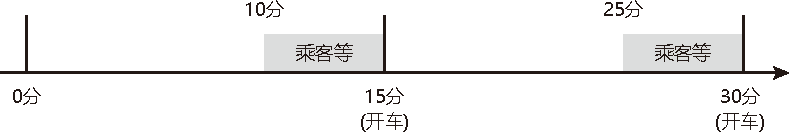
\includegraphics[width=0.8\textwidth]{/0175.pdf} \\
	
	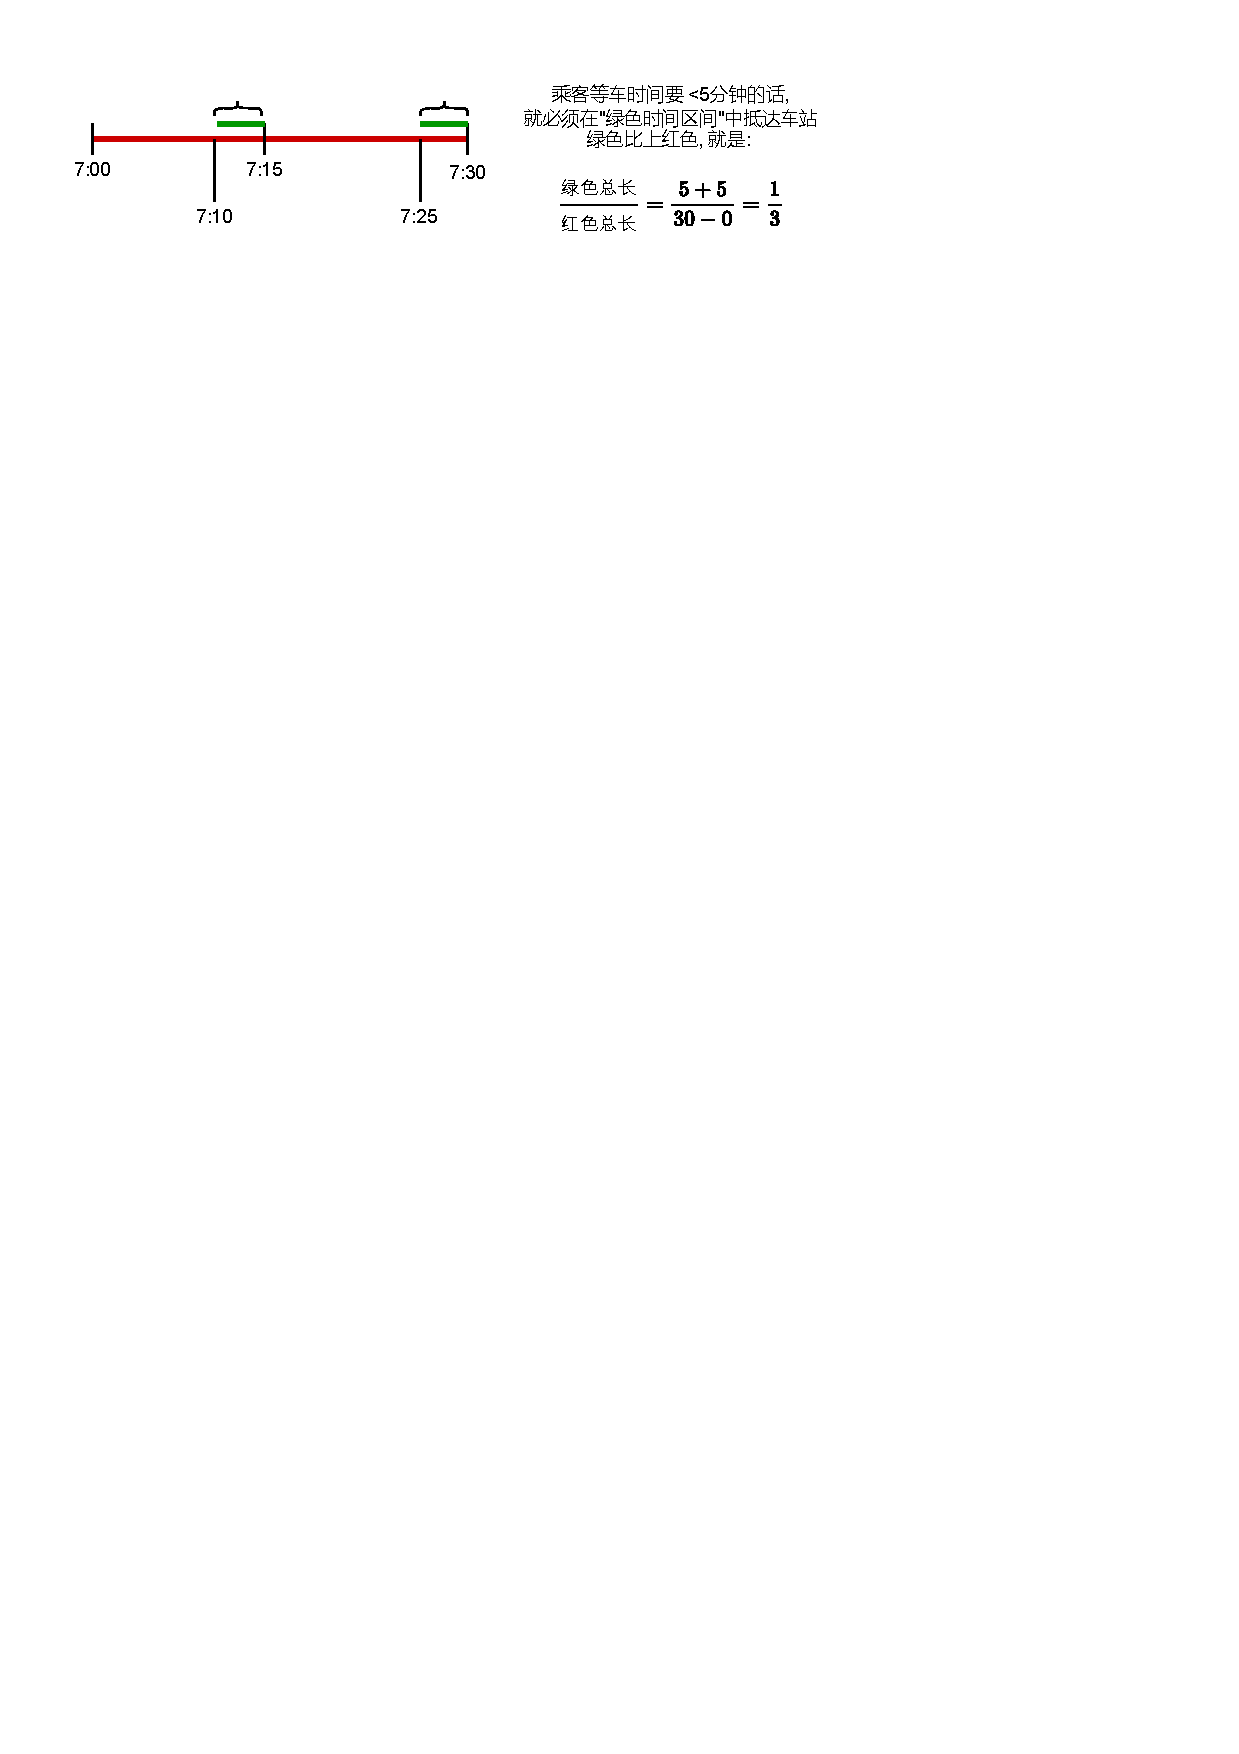
\includegraphics[width=0.8\textwidth]{/0176.pdf} \\
	
	
	\end{myEnvSample}
	
	
\end{document}